\insertmeeting 
	{Capping Craze} 
	{01/24/23} 
	{Hagerty High School}
	{Anouska, Jensen, Jorge, Karissa, Laura, Nathan, Ritam, Robert, Samantha, Tyler}
	{Images/RobotPics/robot.jpg}
	{2:30 - 4:30}
	
\hhscommittee{Hardwhere}
\noindent\hfil\rule{\textwidth}{.4pt}\hfil
\subsubsection*{Goals}
\begin{itemize}
    \item This meeting, one aspect that we discussed was the changes that have occurred in the Team Beacon 

\end{itemize} 

\noindent\hfil\rule{\textwidth}{.4pt}\hfil

\subsubsection*{Accomplishments}
This season we were tasked with a very similar task from last year, capping our team element on a pole. the difference from last year is that this year we are forced to find the easiest way to pick up our element. 
At the beginning of the season, we discussed all the different methods for picking up the team beacon. We began with a handle method where the robot would grip a handle. After a bit of prototyping, we found that this was very slow and had lots of room for improvement
Our second idea was to create a modified cone. We were going to do this by making a hexagonal base instead of a circular base. The problem we found with this was that the cone greatly resembled the original cone element from the field. And secondly, we found that it would be heavy. Finally, we realized that this would be too much work and would not be the most efficient. The rules say that there is a limit on the number of cones you can hold but it does not say that you cannot hold a team beacon and a cone simultaneously.
To capitalize on this new revelation, our third idea was to use slot the beacon onto the cone in order to make it so our robot could grasp onto the cone and the element at the same time.  The first iteration for this element was very rudimentary. It was just a cone cover with our team numbers extruded from the side. This met the requirements for the team element but had two major flaws.
The first major flaw of our initial iteration was the fact that it needed to be bigger. Despite being the minimum size requirement for the team shipping element, 3in x 3 in x 4in, it still would not fit on the cone to allow it to be picked up. This was because the beacon rested on the rib of the cone. To fix this issue, with our next iteration, we would make small indents that would align with the small ribs inside the cone's base.
Our second design iteration was a huge step in the right direction. We were able to make the cone fit between the ribs and this time we were able to lift with it. This was the team element we used at meet 5. Though we didn't get the chance to score the element in a match at meet 5, we learned something crucial about the design. We learned that it is incredibly hard to line up. This is because the notches in the beacon are tiny requiring the human players on the field to be very careful. This means it takes longer and is much more difficult to place the cone on top of the team element.
For our final iteration, we decided to fillet the end of our element in CAD. What that means is that the notches on the beacon will have a smooth transition and will help to guide the beacon into the ribs on the cone. Overall, this final design makes it so our human player does not have to be as accurate when placing the beacon and will allow the robot to fully be able to pick up the beacon while on the cone scoring 18 points if scored on a high pole.
 

\begin{figure}[ht]
  \centering
  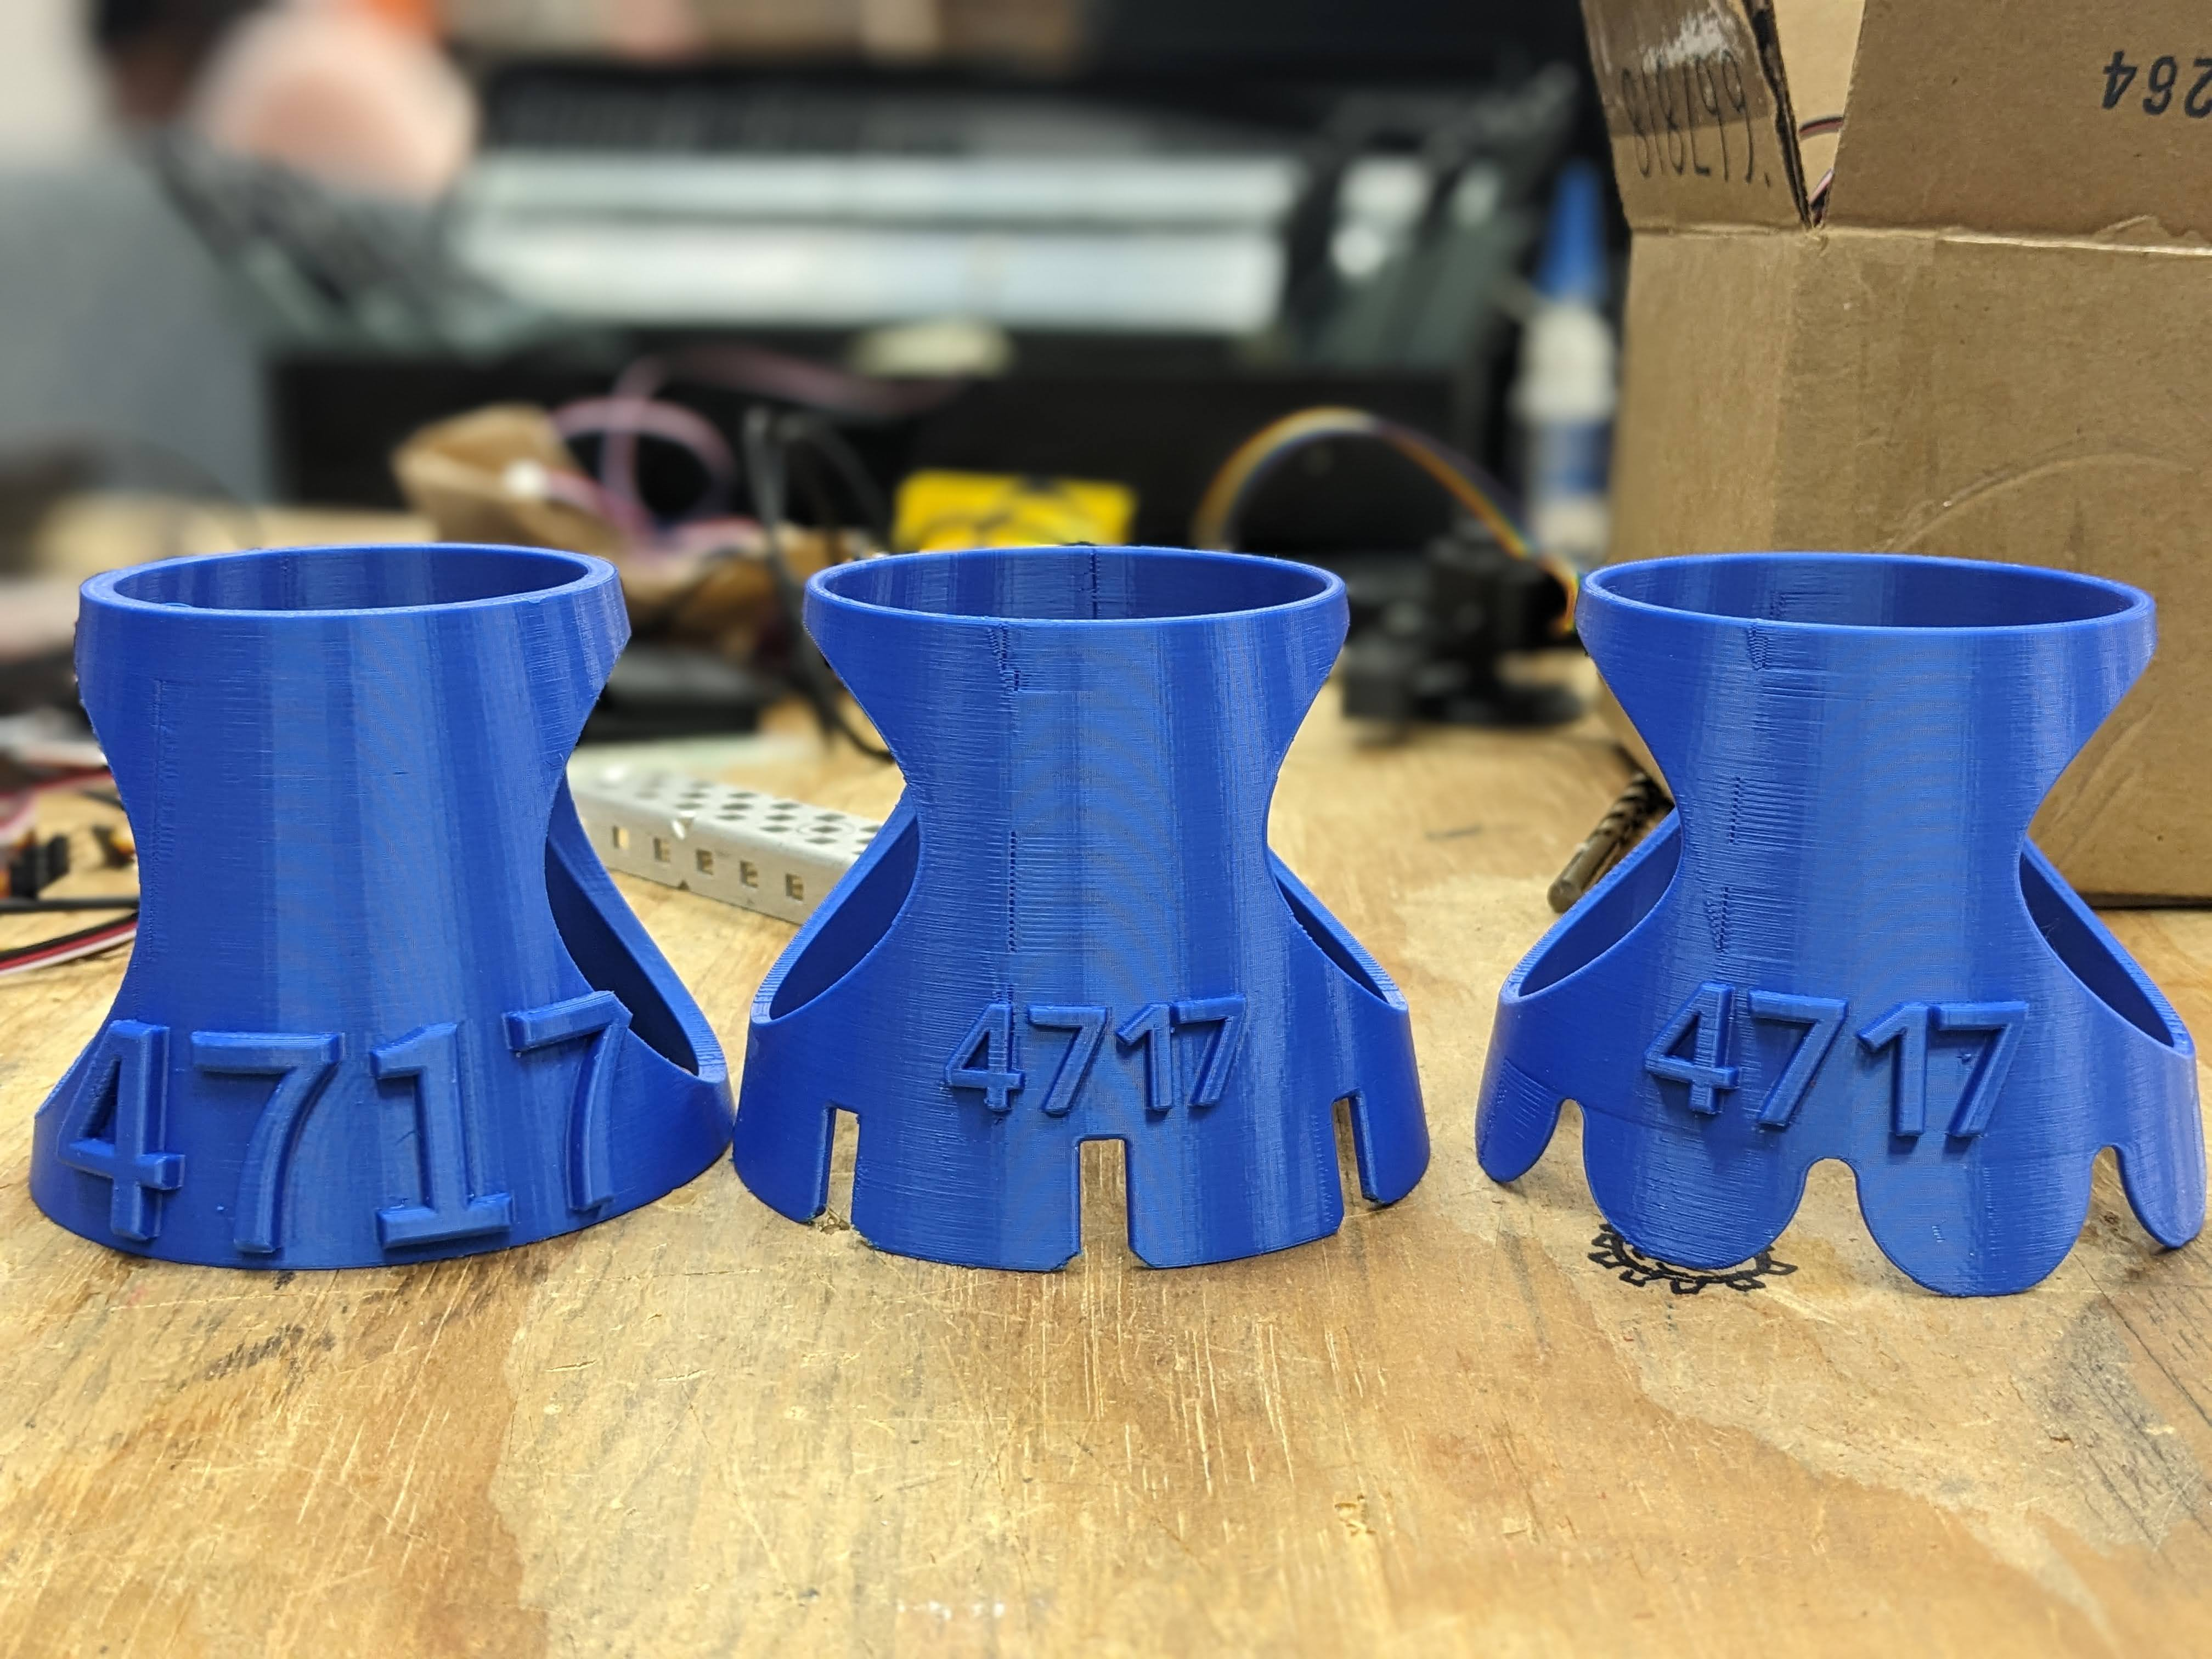
\includegraphics[width=0.95\textwidth]{Meetings/January/01-24-23/01-24-23-TElement.jpg}
  \caption{Old to new variation of team beacon}
  \label{fig:pic1}
\end{minipage}
\end{figure}

\begin{figure}[ht]
  \centering
  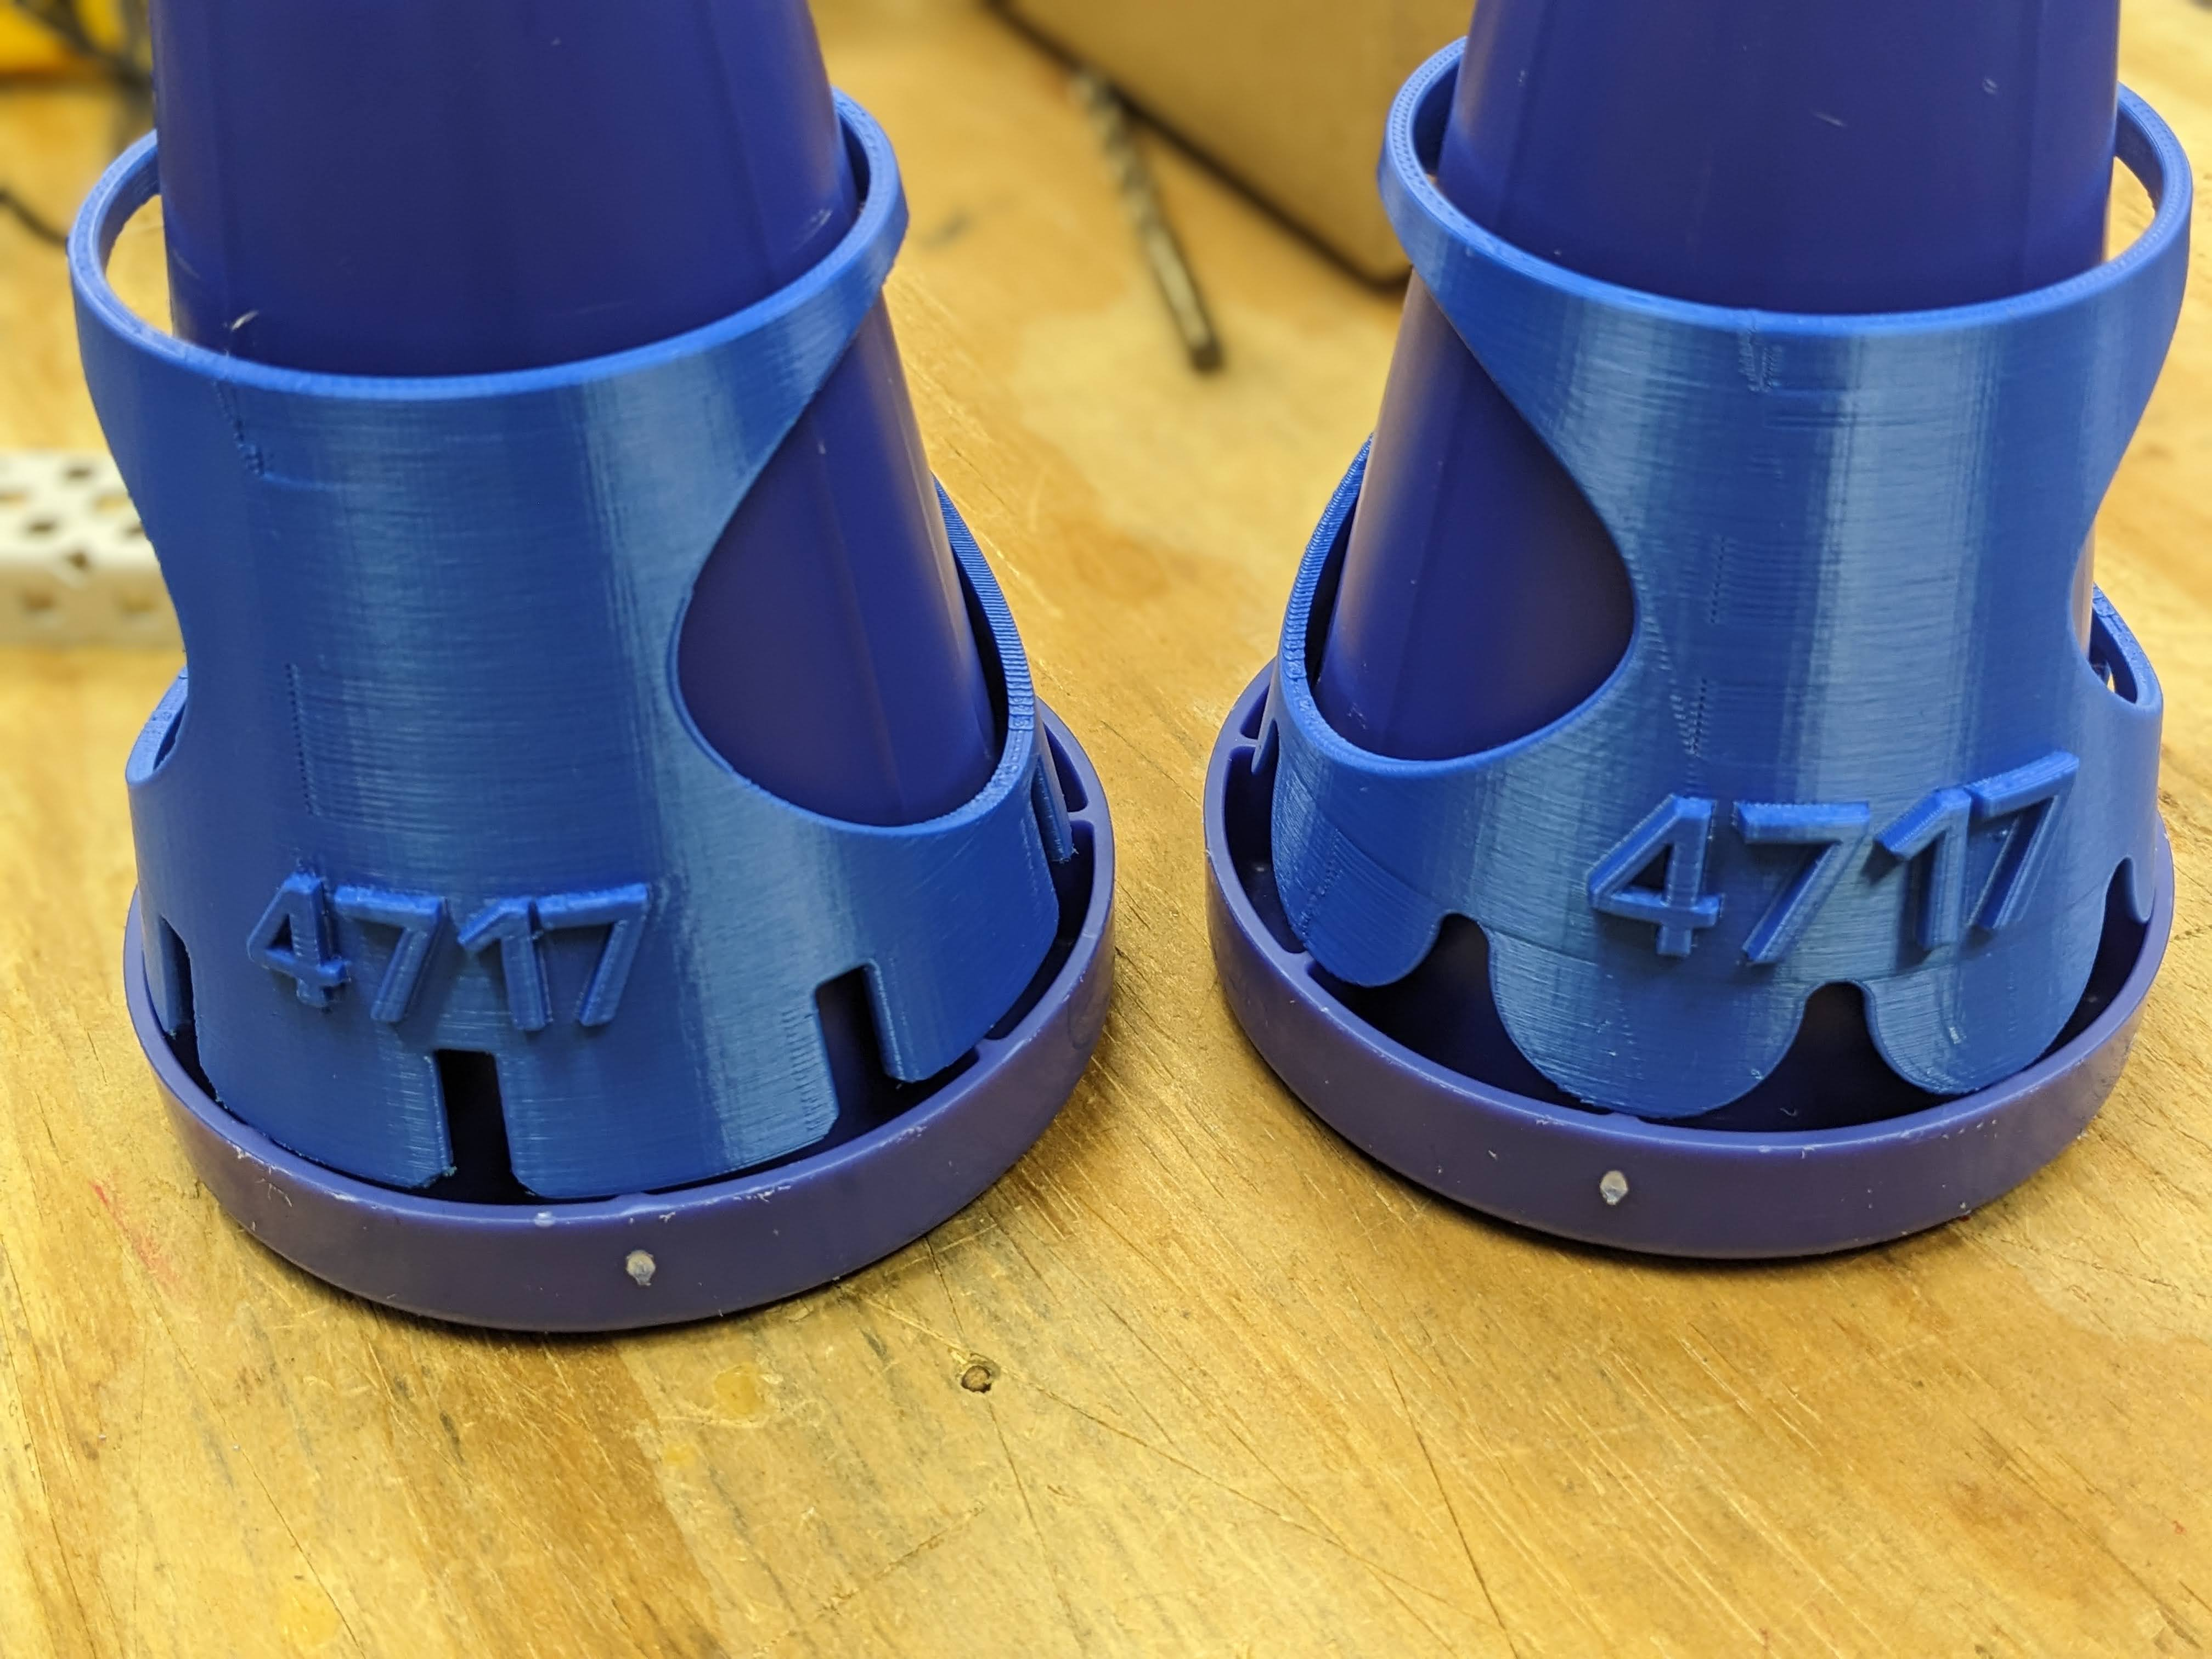
\includegraphics[width=0.95\textwidth]{Meetings/January/01-24-23/01-24-23-TElement2.jpg}
  \caption{Beacon}
  \label{How our new (right) team beacon fits on a cone}
\end{minipage}
\end{figure}


\whatsnext{
\begin{itemize}
    \item Prepare for leagues and modify the Team Element again as necessary
    
\end{itemize} 
}
